% Chapter 6

\chapter{Enigma: A Testbed} 
\label{Chapter6}
\lhead{Chapter 6. \emph{Enigma: A Testbed}} 

\section{Overview and Intentions}

The intention of this project is to produce an application that allows two users to securely identify and authenticate one another, and communicate with text messages via a presumed-insecure network. However, the primary \emph{goal} is to create a testbed that allows any cryptographic algorithms to be integrated in place, to provide a platform for further analysis, such as comparison of run-times between open and closed source implementations.

\section{Engineering Methodologies and Planning}

\subsection{Methodology}

The main focus of the development process was to break the application down in to its component pieces, and iteratively develop them so that minimalist functionality sets could be produced and then combined in the shortest possible times. The overarching category for this style of production is known as \emph{agile development}: a practice based around iterative and incremental development. More specifically, a subset of agile development will be used -- Scrum. The goals of Scrum fit neatly with the desired development cycle in that programming is done in "sprints," with a deadline organised at the start of these sprints and a set of tasks that must be completed by the end. A sprint can last anywhere between one week and one month. This, combined with test driven development (TDD, writing tests for functionality before producing the functionality), produces a set of components matching a well-defined requirements document that can be combined in to the final product.

However, without results, methodologies are meaningless. One should not concentrate too heavily on explicitly following a development process, particularly when working alone, otherwise work output can be reduced significantly by the overhead and ``red tape." Because of this, the methodology of development will not be encountered again in this document, however it is of interest to know the basics as above.

\subsection{Documentation}

Documentation is an extremely important part of software engineering. It is a broad concept, and encompasses: requirements and specification, design overview, technical details, user manuals and even marketing information. However, in terms of the software development process, it is only the first three that are of direct importance. 

It is said a program listing should be documentation unto itself: the programming style should allow an overall structure and purpose to be easily determined from examining the code \cite{McConnell:2004tv}. However, this is an idealistic view and design and technical documentation are of great importance, not only for the developer currently producing the software, but for those possible developers in the future who have to maintain the code.

As a major component of this project is to develop a library of cryptographic algorithms, having a clear and accurate listing of all available methods in the API is vital. Conveniently, Java and the Eclipse IDE are tightly integrated with \emph{JavaDoc}\footnote{http://java.sun.com/j2se/javadoc}, a documentation generator that automatically produces standardised API documentation in HTML format based on comments inserted in the code. The comment blocks -- distinguished using the format \verb!/** ... */! -- contain a method description, and a number of control sequences that give detailed information about what the method returns, the parameters it takes and other details such as exceptions thrown.

JavaDoc outputs are bundled with the appropriate packages in the file tree, and a manual is found in the appendices. A requirements specification has been compiled in \emph{\textsection \ref{AppendixA}}.

\section{Application Development}

  \subsection{User Interface}
  \emph{Packages covered in this section: com.cyanoryx.uni.enigma.gui.*}
  
    \subsubsection{GUI Frameworks}
    
      \paragraph{SWT} -- the Standard Widget Toolkit -- initially created by IBM and now maintained by the Eclipse Foundation, it is a modern alternative to Swing. Initially SWT was used (predominantly in tests) for the Enigma application, however as development continued it became more apparent that it was introducing a level of complexity to the interface code so much so that development slowed to an unmanageable speed. SWT benefits from its use of native component libraries, generally resulting in a more congruent user experience, however it falls down when it comes to ease of development.
      
      \textbf{Pros and cons of Swing}
      
       \begin{center}
       \begin{tabular}{ | p{6cm} | p{6cm} |}
          \hline
          Pros & Cons \\ \hline \hline
          Part of the JDK, meaning there's no need for native system libraries & The look and feel does not always match well with the native system \\ \hline
          No differences in development between platforms and systems & \\ \hline
          Very good documentation available, particularly from Sun & \\ \hline
          Mature and well supported & \\ \hline
          Is supported by official Java extensions like OpenGL & \\
          \hline
        \end{tabular}
      \end{center}
      
      \textbf{Pros and cons of SWT}
      
      \begin{center}
       \begin{tabular}{ | p{6cm} | p{6cm} |}
          \hline
          Pros & Cons \\ \hline \hline
          Uses native components & Native libraries must be available for all supported systems \\ \hline
          Also supported by the Eclipse editor & Some native resources are not available on other systems, and so portability can be damaged \\ \hline
          Documentation is good (though not as good as Swing) & Requires manual management of resources rather than, for example, SWT disposing windows, they must be done by the developer. \\ \hline
          SWT programs can also integrate Swing components & SWT requires separate libraries to be distributed for 32- and 64-bit systems. \\ \hline
          SWT is supposedly faster at rendering than Swing, though only minimally & \\
          \hline
        \end{tabular}
      \end{center}
      
      SWT appears initially simpler to use thanks to its use of the Model--View--Controller design pattern, the ability to ``plug in" different look and feel settings, and so on, however it introduces the necessity to manage resources manually, rather than following the Java standard method of automatic resource disposal (known as the garbage collector).
      
      Swing was selected as the framework to be used, primarily due to its current prevalence over SWT. Purely comparing speed statistics, SWT comes out on top, however the community behind Swing is far larger and more important than the downsides introduced by using Swing, and clearly the balance of pros and cons is in Swing's favour.
      
    \subsubsection{Designs}
    
    Being an application purely for testing purposes, the interface can have a certain leniency in terms of usability as those utilising it will likely have a good understanding of systems anyway. However, more importantly, the interface should be "invisible," meaning that the user should not have to think about using it and can focus on the task they are trying to complete -- e.g. comparing encryption algorithms.
    
    The application will have four main windows:
    
    \begin{enumerate}
      \item Connect Window -- The main starting point of the application. Users will enter the IP address of another Enigma server, or select an address from a ``recently connected" menu.
      \item Chat Window -- Where the actual communications will take place. It will consist of a main listing box to display a message history for the current conversation, and have an input box for sending messages. It will also contain options for: Regenerating session keys, changing the cipher type, changing the agreement cipher type, and viewing the log window for this session.
      \item Log Window -- Can be used to log info, warning and error messages that do not cause a general program crash.
      \item Preferences -- Used to modify basic preferences, like default ciphers, username, etc.
    \end{enumerate}
    
     \begin{figure}
       \centering
       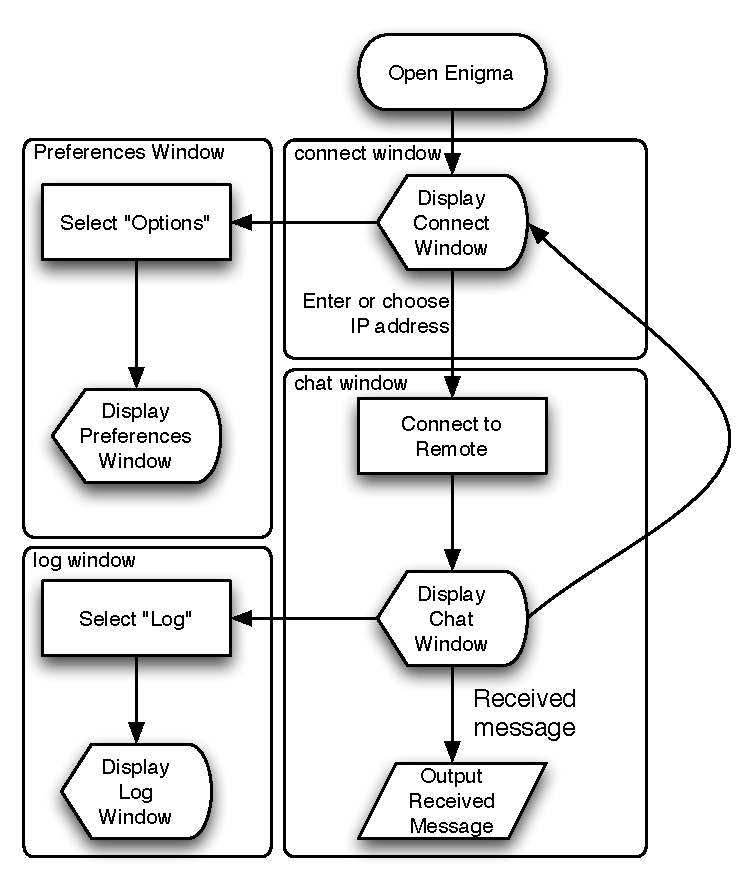
\includegraphics[scale=0.7]{./Figures/Ch6/6-3-1-2a.pdf}
       \caption{Overall Application Flow}
       \label{fig:app_flow}
     \end{figure}
    
    Figure \ref{fig:app_flow} shows a basic overview of how the application will be used.
    
    As developed with Swing, the four main windows look as so (on Mac OS X):
    
    \subsubsection{Connect Window}
    
    \begin{figure}
      \centering
      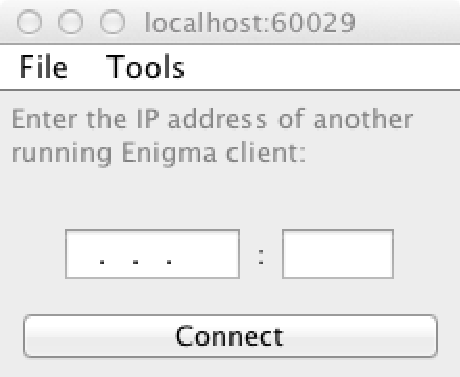
\includegraphics[scale=0.7]{./Figures/Ch6/6-3-1-2-connect_window.pdf}
      \label{fig:connect_window}
    \end{figure}
    
    The Connect window comprises of two main pieces of logic:
    
    \begin{enumerate}
      \item Server creation.
      \item Connection making.
    \end{enumerate}
    
    Firstly, the Connect window is the main focal point of the application and as such the creation of a \verb!Connect! object signifies the start of the Enigma application. \verb!Connect#Connect()! creates a new \verb!Server! object with a random port number and initiates the process of creating the UI for the window.
    
    As with most Swing-utilising classes, event handlers are used to process events triggered by user input -- such as a button press -- and in this case the main event handler will be that of the connect button. When a valid IP address is input and the button is clicked, the \verb!connect()! method is run: \\
    
    \begin{lstlisting}
private void connect(String address, String remote_port) {
  try {
    // Display a loading screen
    Connect.this.showLoading();
    
    // As we are the initialiser,
    // generate a session ID
    String id = ""+(new Random().nextInt(100));
    
    // Create a new Session to store data for the remote server
    Session session = Server.createClient(address,
                      remote_port,
                      ""+port,
                      new User("remote user"),
                      id);
                      
    // Store the Session in the server's session index
    Connect.this.server.getSessionIndex().addSession(session);

    // Send our desired agreement method
    session.sendAuth("method",
                     "agreement",
                     new AppPrefs().getPrefs()
                                   .get("default_asym_cipher","RSA"),
                                        id);
                                        
    // Send our public key and certificate
    session.sendAuth("cert",
                     "agreement",
                     Base64.encodeBytes(new Certificate(
                                            new File("./cert"))
                                            .toString()
                                            .getBytes()),
                     id);
    
    // Store the remote server's IP address
    new AppPrefs().getPrefs().put("last_connections",
                   address+":"+port+";"+new AppPrefs().getPrefs()
                                   .get("last_connections",""));
  } catch (Exception e) {
    [...] // Display an error
  } finally {
    try {
      // Always reinstate the UI
      Connect.this.recreateUI();
    } catch (ParseException e) {
      e.printStackTrace();
      System.exit(1);
    }
  }
}
\end{lstlisting}
    
    Here we make use of a method \verb!Server#createClient()!, which is a bit of a misnomer based around a legacy concept within the application where a local user would run both a server and a ``client," for sending and receiving data, respectively. This was designed as such due to some restrictions on the use of sockets, however this was removed for simplicity and due to the confusion introduced by running a ``client" locally.
    
    \verb!Server#createClient()! is a simple, static method that creates a \verb!Session! object with the supplied attributes and returns it, along with a \verb!Conversation! object for the chat window.
  
    \subsubsection{Chat Window}
    \label{subsubsec:chat}
    
    \begin{figure}
      \centering
      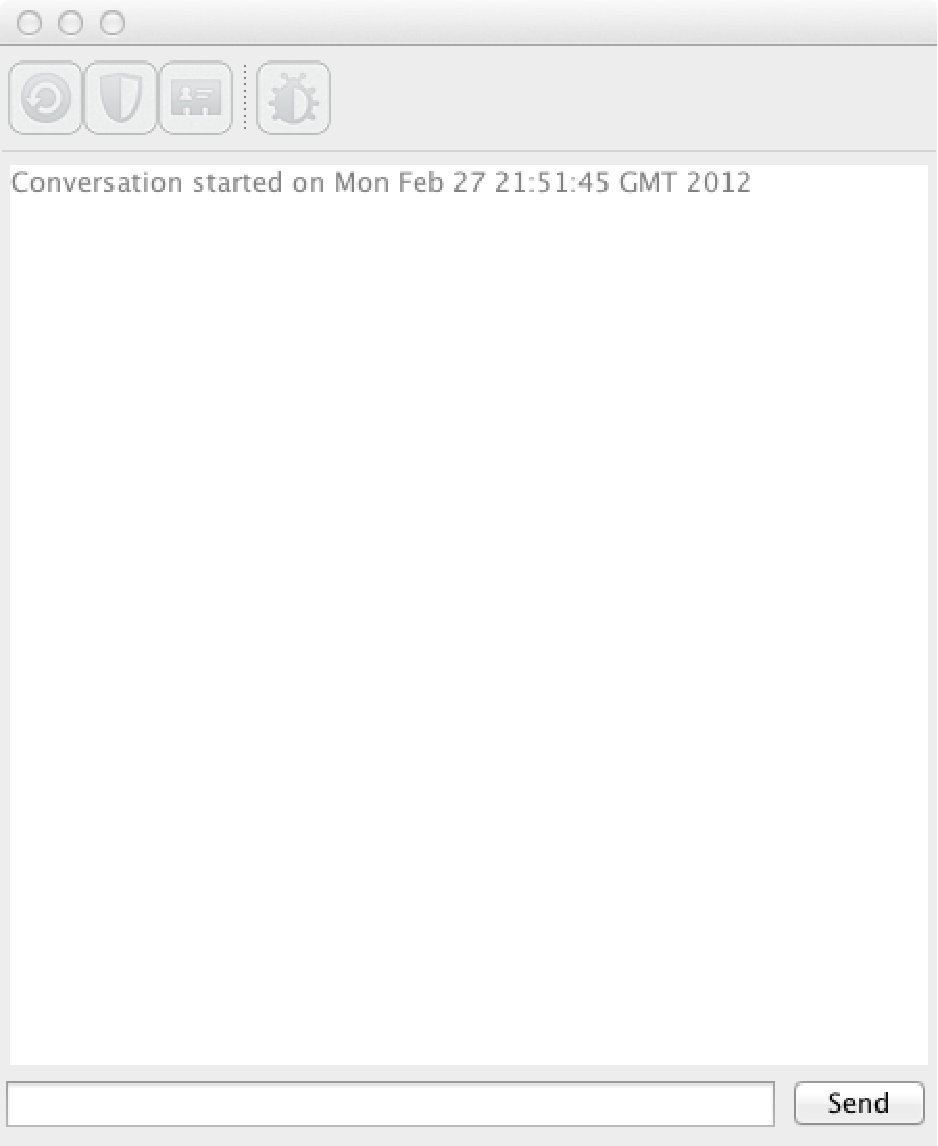
\includegraphics[scale=0.7]{./Figures/Ch6/6-3-1-2-chat_window.pdf}
      \label{fig:chat_window}
      \caption{Chat Window}
     \end{figure}
    
    The conversation has three tasks:
    
    \begin{enumerate}
      \item Display received messages.
      \item Take the user's input and send the message to the relevant \verb!Session! object for encryption and transmission, and then display that message in the window (if sent).
      \item Provide access to the following functionality:
        \begin{enumerate}
          \item Opening/closing the log window.
          \item Regenerating the session keys.
          \item Viewing the remote user's certificate.
          \item Toggling encryption on and off.
        \end{enumerate}
    \end{enumerate}
    
    Each are relatively simple as most of the hard work is handed off to other objects within the \verb!Server!'s jurisdiction. 
    
    \paragraph{The display of messages} is implemented using a \verb!JTextPane! which, unlike a \verb!JTextArea!, honours the use of font styling, colours and post-creation programmatic string insertion. The \verb!updateMessage()! method takes a user name and a message: \\
    
    \begin{lstlisting}
public synchronized void updateMessage(String name, String message)
                 throws BadLocationException {
  StyledDocument d = messages.getStyledDocument();
      
      SimpleAttributeSet kw = new SimpleAttributeSet();
      StyleConstants.setBold(kw,true);
      
  d.insertString(d.getLength(),name+": ",kw);
  // Use a blank attribute set for the actual message text
  d.insertString(d.getLength(), message+"\n", new SimpleAttributeSet());
}
\end{lstlisting}
    
    Two new Java classes are required: \verb!StyledDocument! and \verb!SimpleAttributeSet!. The former converts the messages \verb!JTextPane! in to an object that can be formatted, and the latter is a set of attributes that can be applied as formatting to the text we are appending to the text pane. 
    
    \verb!Conversation! windows are somewhat different from other interfaces in that they are persistent to a connection -- conversations windows are stored in \verb!Session! objects (as we will see later). Because of this, when a message is received, the handler retrieves the \verb!Conversation! object and calls \verb!updateMessage()!.
    
    \paragraph{Sending messages} is handled entirely by \verb!Session! objects, and so when a user enters text and hits enter or clicks "send," the \verb!Session#sendMessage()! method is called.
    
    Displaying the log window, viewing the remote user's certificate and regenerating the session keys are all similarly simplistic in their implementation. The latter utilises the \verb!Session#sendAuth()! method to regenerate a key and send it, however this is discussed in detail later. The other two buttons simply toggle the current display status of the two windows.
    
    Toggling the encryption status is slightly more complex, however. The current status of encryption for the conversation must be checked, and turning it on or off depending on the result, also checking if the user allows for unencrypted conversations.
    
    \subsubsection{Log Window}
    
    \begin{figure}
      \centering
      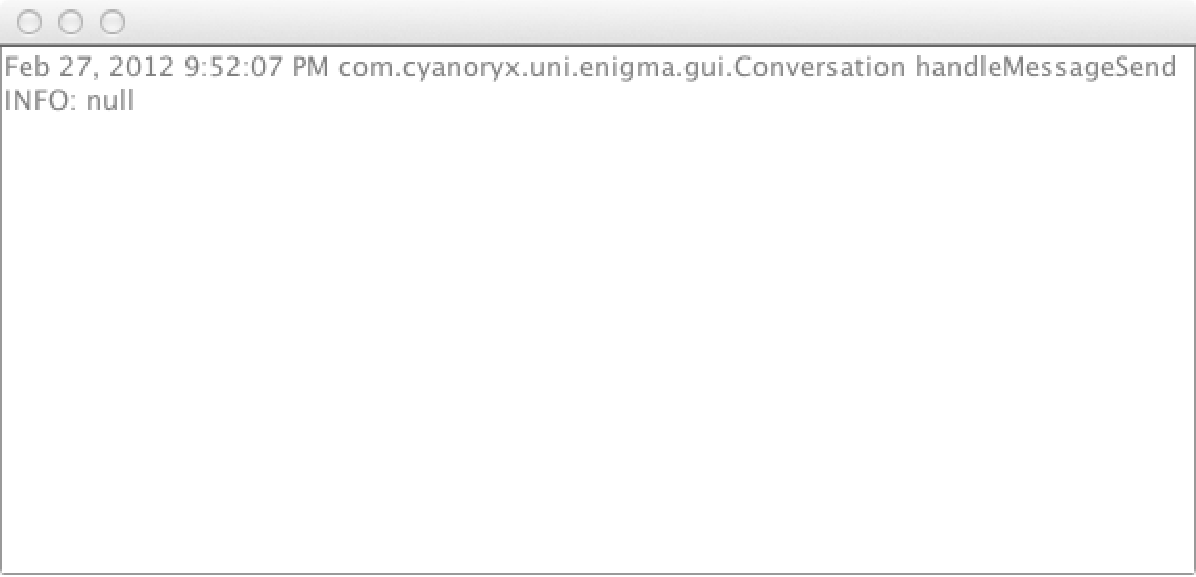
\includegraphics[scale=0.5]{./Figures/Ch6/6-3-1-2-log_window.pdf}
      \label{fig:log_window}
      \caption{Log Viewer}
     \end{figure}
    
    The log window itself is a simple setup (\verb!LogWindow!): a Swing \verb!JFrame! wrapper with a disabled \verb!JTextArea! and a method for handling input to be appended to the text area. The complexity behind it, however, is in the \verb!LogHandler! class. \verb!LogHandler! extends \verb!java.util.logging.Handler!, but why not just have a \verb!LogWindow! object and have each class manually update the text area? Using a \verb!Handler! implementation is all about \emph{extensibility}: it provides built-in capability for handling logging level settings (e.g. only log warnings, information, errors, etc.), along with applying formatters and filters. In the current version of Enigma, only the \verb!Conversation! class needs to log information and so the log handler does little data modification and simply passes the messages on to a \verb!LogWindow! object.
    
    For the full code behind the logging system, see \emph{com.cyanoryx.uni.enigma.gui.Log*.java}.
    
    \subsubsection{Preferences Window}
    
    User preference changed are handled by a single, unified preferences window, created by a \verb!com.cyanoryx.uni.enigma.gui.Preferences! class (which should be distinguished from \verb!Preferences! in the \emph{java.util.prefs} namespace). It is another simple class that implements a \verb!JFrame! containing multiple \verb!JTabbedPane! elements separating out preferences in to their relevant categories. 
    
     \begin{figure}
      \centering
      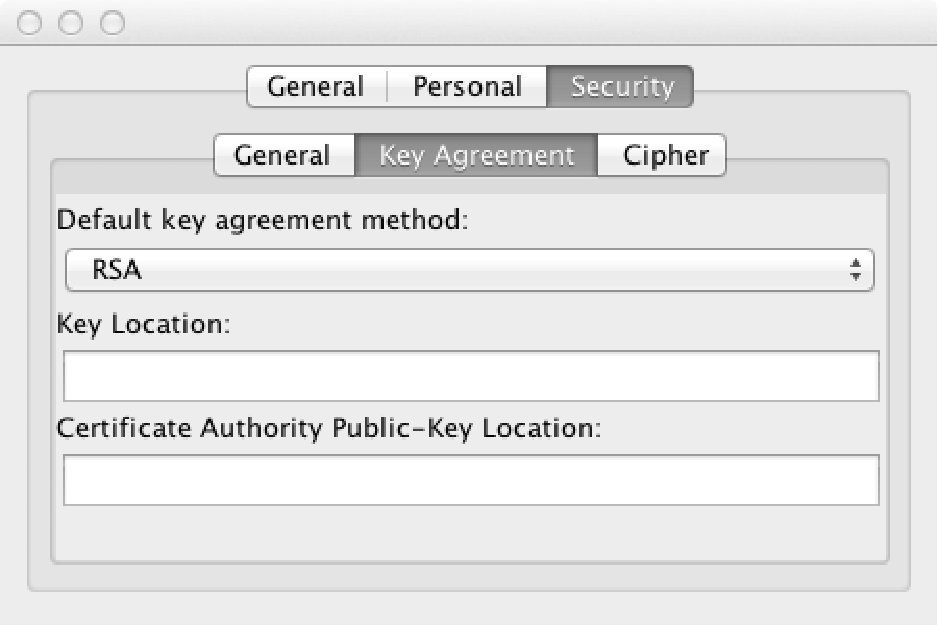
\includegraphics[scale=0.7]{./Figures/Ch6/6-3-1-2-preferences_window.pdf}
      \label{fig:pref_window}
      \caption{Preferences}
     \end{figure}
    
    Upon loading, each preference component is created with its value equal to the currently stored value, or if there is none, a default value. Each preference is governed by an event listener appropriate to the data type of the option:
    
    \begin{enumerate}
      \item \verb!ItemListener! -- boolean preferences use \verb!ItemListener#itemStateChanged()! to register for a checkbox state change.
      \item \verb!ActionListener! -- preferences with multiple choices implemented as drop down combo boxes register with \verb!ActionListener#actionPerformed()! to monitor item selection.
      \item \verb!DocumentListener! -- string based preferences, such as user name, are monitored using the update registering methods in \verb!DocumentListener! to detect updated, deleted or inserted text.
    \end{enumerate}
    
    When an event is generated, the updated preference is stored, meaning that the user never has to press any ``save" or ``apply" buttons.
    
    In the future, it would perhaps be interesting to retrieve the list of available settings and their datatypes, and automatically generate a preference interface based on this. However, this may pose problems for preferences with multiple choices (like in drop down boxes), as all the options will not be saved in the preferences storage.
    
    See \textsection\ref{subsec:prefs} for the actual implementation of preference storage.
    
    Each window was developed using the Swing framework, as mentioned, but the "look and feel" of the components were designated to match the JDK's interpretation of the system's theme, meaning that the components will be very similar to those used in native applications thus making the application more portable, at least in terms of appearance. 
    
  \subsection{Preferences}
  \label{subsec:prefs}
  
  It is necessary to have some persistent data between application sessions, for example the user's display name and their cipher preferences. There are many simple and many complex methodologies to solve this problem, the simplest seemingly being saving preferences to a text file with a custom format. However, as with any proprietary format it will be non-portable from the outset, and likely difficult to maintain in the future. Large amounts of ``boiler--plate" code will be required to manage aspects like text-encoding, storage location, file formats, and so on which will unnecessarily add to development time and likely create bugs.
  
  The JDK comes with a class \emph{com.util.prefs.Preferences} for storing a collection of preference data. \verb!Preferences! stores data in a key-value persistent backing store that is independent of the system implementation. Given a ``node" name, \verb!Preferences! will load data from the appropriate storage implementation, depending on the operating system. For example, it may store preferences in flat files, registries or even databases. This has one primary benefit: the developer does not need to concern themselves with the details of storage, but merely implement an application that creates a \verb!Preferences! object given a node name and \verb!Preferences! will handle the details.
  
  More specifically, \verb!Preferences! has a static method \emph{userNodeForPackage(String name)} which returns a \verb!Preferences! object containing handles that reference the persistent backing store. This \verb!Preferences! objects provides helper methods such as \emph{get(String key, String default\_val)} that will programmatically return the value for the key \verb!key!, handling any errors and using the default value if necessary. 
  
  However, this introduce an integrity and consistency issue: what if the node name changes? Do we store the node name in a centralised location? (introducing something of a chicken and egg problem). Or perhaps assume that it will never need to change? In our case, a wrapper class was created that returned a \verb!Preferences! object with a node name equal to \verb!getClass()!. This way the node will always be named after the package identifier for the given class, which can be refactored if necessary. \\
  
  \lstinputlisting{../../sys/EnigmaApp/src/com/cyanoryx/uni/enigma/utils/AppPrefs.java}
  
  \emph{This code can be found in com.cyanoryx.uni.enigma.utils.AppPrefs}
  
  We have also written a helper method that returns the last 10 IP connections, which are stored upon connection as a concatenated \verb!String! array.
  
    \subsubsection{Usage}
    
    \begin{lstlisting}
Preferences p = new AppPrefs().getPrefs();
p.get("preference_name","test");
\end{lstlisting}
  
  \subsection{Internationalisation}
  
  Internationalisation, colloquially shortened to \emph{i18n} as 18 is the number of characters between the first and last letters, of an application is adding the possibility of easily creating new language sets that allow components and text in the application to be translated and shown in another language while retaining the ability to switch back to other languages. The purpose is to remove the need for software changes, and introduce a preference or setting that points the application to appropriate language set.
  
  In this case, the language sets are stored in \verb!.properties! files: \\
  
  \lstinputlisting{../../sys/EnigmaApp/bin/Enigma.properties}
  
  As with the preferences, a helper class is necessary to access the locale information and abstract some of the more verbose syntax needed for getting language information. In this case, a class \verb!Strings! has been created that on initialisation gets the locale preference and attempts to load the corresponding language set (known in \verb!Locale! parlance as a bundle), and provides a translate method that takes a string identifier, and returns the matching language string from the current locale bundle. \\
  
  \lstinputlisting{../../sys/EnigmaApp/src/com/cyanoryx/uni/enigma/utils/Strings.java}
  
  \emph{This code can be found in com.cyanoryx.uni.enigma.utils.Strings}
  
  \subsection{Drawable Graphics}
  
  Some elements of the user interface require the inclusion of local images and icons. For example, in the chat window the menu bar buttons contain representative icons rather than text. However, as with strings of text, hard-coded references to resources generally results in excessive maintenance if the resource location changes. As a solution to this, we will create a lightweight class modelled around the \emph{Android SDK} concept of ``drawables." Drawables are graphic resources stored in the system, represented by an identifier which can be retrieved using the \verb!Drawable! class.\\
  
  \lstinputlisting{../../sys/EnigmaApp/src/com/cyanoryx/uni/enigma/utils/Drawable.java}
  
  \emph{This code can be found in com.cyanoryx.uni.enigma.utils.Drawable}
  
  As an example: if we decide that a database is more suitable for storing graphics than local files, the \verb!loadImage()! method can be modified to search the database for the identifiers, and all the (possibly) hundreds of references to images within other parts of the codebase will not have to change.

\section{Protocol Implementation}
  \emph{Packages covered in this section: com.cyanoryx.uni.enigma.net.*}
  
  \subsection{Overview}
  
  The purpose of the Enigma application is to provide an example application to be used for testing cryptographic algorithms, however the \emph{function} of the application is to provide a means of communication between two entities who are capable of running the same software. To do this we will be implementing a custom variation of the Jabber/XMPP protocols within a server that will be able to send and receive  XML data streams.
  
  Servers are simple to implement, particularly with Java's excellent networking support -- simply open a port locally that accepts connections, and parse any input and return outputs where necessary. However, there are many other aspects of running a server that are not covered by this in any form: for example, handling multiple connections efficiently and reliably, maintaining message integrity, and so forth. Because of this, we will be creating a server that is extensible and advanced in how it deals with connections and input. Alongside this, by introducing XML parsing capabilities and a well-defined protocol we are able to improve reliability (by being able to detect malformed XML) and make handling different types of input easier (by have distinct sets of XML tags for specific purposes).
  
    \subsubsection{Goals and Objectives}
    
    \begin{enumerate}
      \item Simplicity -- the server should have components which are only strictly necessary. Very little time should be spent on input processing.
      \item Easy to integrate with cryptographic algorithms -- this is harder to quantify, however it should result in software where there are only a small handful of points where algorithms will need to be connected, reducing the amount of repetition.
      \item Extensible -- it should be easy to add new handlers in the event the protocol is modified.
    \end{enumerate}
    
    For a full requirements specification, see \textsection \ref{AppendixA}.
    
  \subsection{Server Design}
  
    \subsubsection{Server}
    
      \begin{figure}
        \centering
        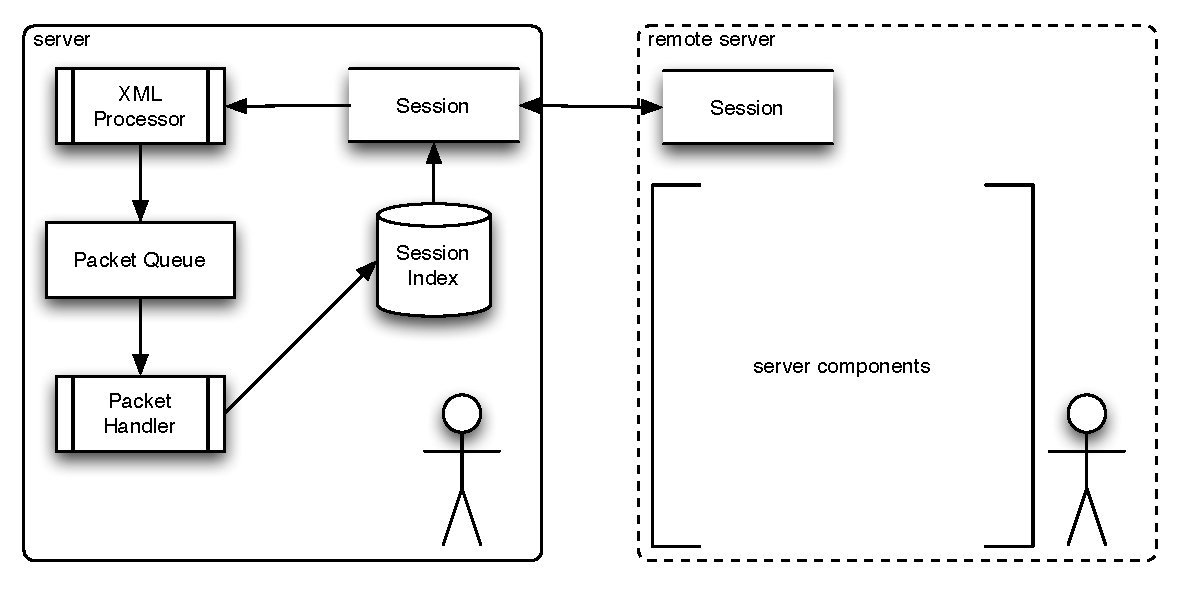
\includegraphics[scale=0.7]{./Figures/Ch6/6-4-2.pdf}
        \caption{A simplified overview of two servers communicating.}
        \label{fig:server_overview}
      \end{figure}
      
    The server is be split in to four major components:
    
    \begin{enumerate}
      \item Sessions -- connections between two entities will be managed by \verb!Session! objects stored in an index.
      \item Packets -- packets represent sections of an XML document are stored in a queue upon arrival, and are handled in a first come first served basis by the XML parser.
      \item XML parser -- the XML parser takes packets and converts them in to Java objects for use in handler endpoints.
      \item Handlers -- after a packet has been parsed, it is sent to the registered handler for its type, which processes the packet. For example, a message handler would only take \verb!<message>! packets and would send them to the correct GUI window for the sending entity.
    \end{enumerate}
    
    Various threads will be created to allow for concurrent processing of multiple connections, however all these threads will run under a parent \verb!Server! thread that maintains connections and sessions, along with dealing with registering packet handlers.
    
    The server uses \verb!java.net.ServerSocket! to create a socket that accepts all connections on a specified port. The port is defined during object construction, generally it should be random, and \verb!Server! will throw an \verb!IOException! if the port is already taken.
    
    \subsubsection{Session}
    
    The \verb!Session! and \verb!SessionIndex! classes form the basis around managing connections between servers -- a \verb!Session! object represents a single connection between two entities. \verb!Session! objects store a number of bits of information regarding a connection that provide context, such as the connection ID (for use in sending messages to the correct GUI window), the \verb!java.net.Socket! associated with the connection, the stream objects for sending/receiving data, statuses, and so on. A \verb!Session! object is created upon connection and filled with the relevant data (random connection ID, user details, etc.) and as long as the connection remains open the \verb!Session! object will remain in memory.
    
    However, Java objects are transient and cannot be easily transmitted across a network, particularly using XML. The \verb!Server! maintains an objects called \verb!SessionIndex!, which is a wrapper around a \verb!java.util.Hashtable! where the key is the connection ID (also referred to as a session ID) and the value is the corresponding \verb!Session! object. By doing this, we are able to maintain a persistent store of information regarding a connection that is easily accessible from all objects within the \verb!Server!, like packet handlers.
    
    The \verb!Session! is also used to store, upon connection, a \verb!Conversation! object for the newly opened conversation window. Upon receipt of a \verb!<message>!, the message handler will look up the session using the session ID received with the packet, and use methods within the \verb!Conversation! object to update the window with the received message.
    
    As local \verb!Session! objects are created by the server when a outbound connection attempt is made, they are used to handle the assembly and transmission of packets, such as connection packets, message, authentication, etc.
  
  \subsection{Protocol Model}
  
  \emph{For structural information regarding the protocol, see \textsection \ref{AppendixB}.}
  
  The protocol model is based around using XML (eXtensible Markup Language) to transmit data along with metadata (attributes) to represent instructions to be received by another system.
  
    \subsubsection{Routing and How It Works}
    
    We will find out in this section how packets are routed through the server upon receipt, along with how they are sent. Figure \ref{fig:conv_overview} provides an overview of how two entities will communicate with one another, and what packets are required.
    
    \begin{figure}
      \centering
      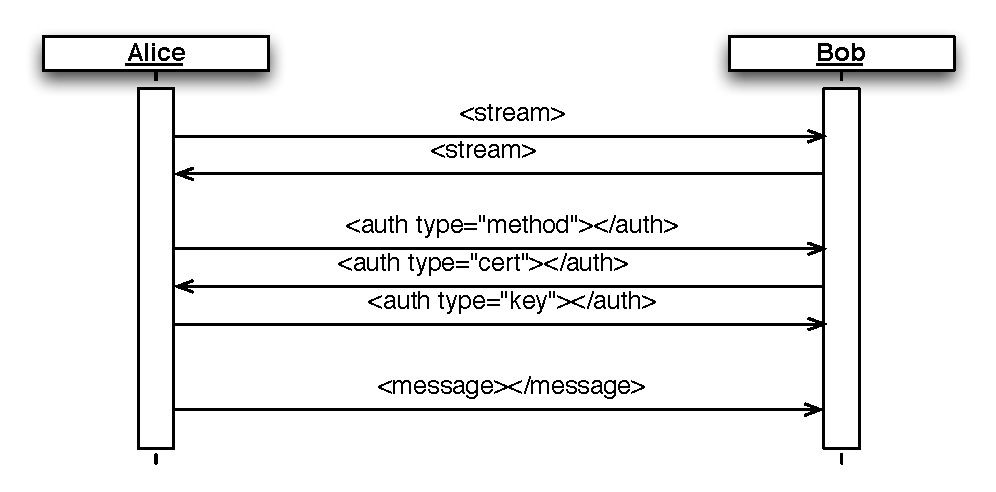
\includegraphics[scale=0.7]{./Figures/Ch6/6-4-3-1.pdf}
      \caption{The basic conversation elements between two entities.}
      \label{fig:conv_overview}
    \end{figure}
    
  \subsection{Parsing XML}
  
  Before we can start converting received messages in to Java objects and handling them, we must parse the XML in to something more usable.
  
    \subsubsection{SAX and Xerces}
    \label{subsubsec:sax}
    
    An implementation of the Simple API for XML (SAX) known as Apache Xerces is used as the SAX parser for incoming packets. Originally a Java-only library, it has become the standard for XML parsing within Java. It uses an event-driven model to parse XML documents, and rather than handling entire documents at once, it is done in a continuous stream of pieces, unlike DOM parsers (Document Object Model) which run using trees based on a complete document. The benefits of this for us are three-fold:
    
    \begin{enumerate}
      \item It is considerably faster than standard parsing, and works in linear time.
      \item Only small portions of a document need be in memory at any one time, and so the memory footprint of parsing a document is small.
      \item It can handle not being in possession of a full, valid XML document  when parsing, like the packets we will be sending between entities.
    \end{enumerate}
    
    It has one primary downside however: developer time. The concept of event-driven XML parsing is harder to manage than simply imagining a document as a tree. However, using Apache Xerces significantly improves upon this as the developer no longer has to handler the parsing itself, but merely what to do with the data once it is parsed. Xerces is more accurately a modular library for parsing, validating and manipulating XML documents. It introduces a framework known as \emph{Xerces Native Interface} that allows developers to build their own parser components, however we will only be using it for its SAX features.
    
    SAX parsers will follow through a document, and upon reaching specific points it will generate events and execute a callback function. For example, upon reaching the start of an element -- e.g. \verb!<message>! -- the parser could be configured to call a function \verb!startElement()! that determines what to do with this new element.
    
    One interesting thing to note is the use of the class \verb!StreamingCharFactory!. While capable of handling subsections of XML documents, SAX parsers are not generally (by default) able to handle streaming data as it arrives, and so the parsers will hang until reaching the end of the document (in this case, the connection closes). \cite{Shigeoka:2002ys} details the \verb!StreamingCharFactory! class that configures Xerces to use a streaming data reader rather than the default buffered one.
    
    \paragraph{The InputHandler} class deals with XML parsing by processing these SAX events. The primary way that documents will be handled is through \emph{depth} -- each section of the document is treated as a tree (as in DOM parsing). Upon encountering each element, the depth is increased by one, and decreased by one when the element ends. This is known as depth-first searching. We have three main methods that handle events:
    
    \begin{enumerate}
      \item \verb!startElement([...])! -- aptly named method that handles the start of elements.
      \item \verb!characters(char[] c,int start,int length)! -- handles the string values of elements.
      \item \verb!endElement(String uri,String localName,String name)! -- handles the closing tags for the current open element. 
    \end{enumerate}
    
    Methods 1 and 2 create \verb!Packet! objects that represent their respective XML elements. In the case of \verb!startElement()!, when at depth 0 the only element possible is a root \verb!<stream>! and so a \verb!Packet! with element name ``stream" is created and pushed on to the queue, along with the attributes passed down from the SAX parser: \\
    
    \begin{lstlisting}
public void startElement(String namespace,
                                 String localName,
                                 String name,
                                 Attributes attributes)
                     throws SAXException {
  switch (depth++){
    case 0: // Root element
      if (name.equals("stream")){
        Packet packet = new Packet(null,name,namespace,attributes);
        packet.setSession(session);
        packet_queue.push(packet);
        return;
      }
      throw new SAXException("Root element must be <stream>");
    case 1: // Message elements
      packet = new Packet(null,name,namespace,attributes);
      packet.setSession(session);
      break;
    default: // Any child elements
      Packet child = new Packet(packet,name,namespace,attributes);
      packet = child;
  }
}
    \end{lstlisting}
    
    As can be seen, at depth 1 a \verb!Packet! is created with all the provided attributes from the parser, including the name. At any other depth, however, we can assume we are dealing with a child element and so the previous \verb!Packet! is set as its parent (see \textsection\ref{subsubsec:packets} for details about how parent-child relationships are implemented programmatically) and all other attributes are stored as usual. At each depth, a global \verb!Packet! object is stored in the class to give access child packets access to parents.
    
    If we are dealing with a value of an element, for example the body of a message, the method \verb!characters()! is called by the parser. \verb!characters()! is a simple method that adds a child value to the last traversed packet in the tree. \\
    
    \begin{lstlisting}
public void characters(char[] c,int start,int length) throws SAXException {
  if (depth > 1) packet.getChildren().add(new String(c,start,length));
}
    \end{lstlisting}
    
    Finally, when an end element is reached we will once again check the current depth. If it is of depth 0, we must be at the end of the document and so a \verb!</stream>! packet is created and pushed on to the queue. At depth 1, the current packet is complete and can be pushed on to the queue, and otherwise we must still be assembling the parent, and so set the pointer to the parent packet. \\
    
    \begin{lstlisting}
public void endElement(String uri,
                            String localName,
                            String name)
       throws SAXException {
  switch(--depth){
    case 0: // End of the stream
      Packet c_packet = new Packet("/stream");
      c_packet.setSession(session);
      packet_queue.push(c_packet);
      break;
    case 1: // Put the completed packet on the packet queue
      packet_queue.push(packet);
      break;
    default:  // Parent still being constructed; traverse back up the tree
      packet = packet.getParent();
  }
}
    \end{lstlisting}
    
    \subsubsection{Packets}
    \label{subsubsec:packets}
    
    All packet related classes can be found in \emph{com.cyanoryx.uni.enigma.protocol.xml}.
    
    Packets in the context of the Enigma protocol are somewhat distinct from what are traditionally known as packets in networking. When we refer to packets we are referencing the XML sections representing messages sent between entities. In the previous section, \textsection\ref{subsubsec:sax}, we defined how these XML fragments are parsed and converted in to packets without really defining what a packet in this context is (henceforth any references to ``packet" will refer to the concept of sections of XML, unless stated otherwise or defined as a class, e.g. \verb!Packet!). Previously we described creating packets by instantiating \verb!Packet! objects with the name, attributes and child elements of the XML -- this class serves two purposes:
    
    \begin{enumerate}
      \item To provide the capability of storing packets internally and in memory without the need to re-parse each time the data is needed, and to provide helper methods to retrieve this data.
      \item To allow the simple, programmatic creation of XML packets through the instantiation of \verb!Packet! objects which can then be converted in to XML to be transmitted across the network.
    \end{enumerate}
    
    \begin{center}
      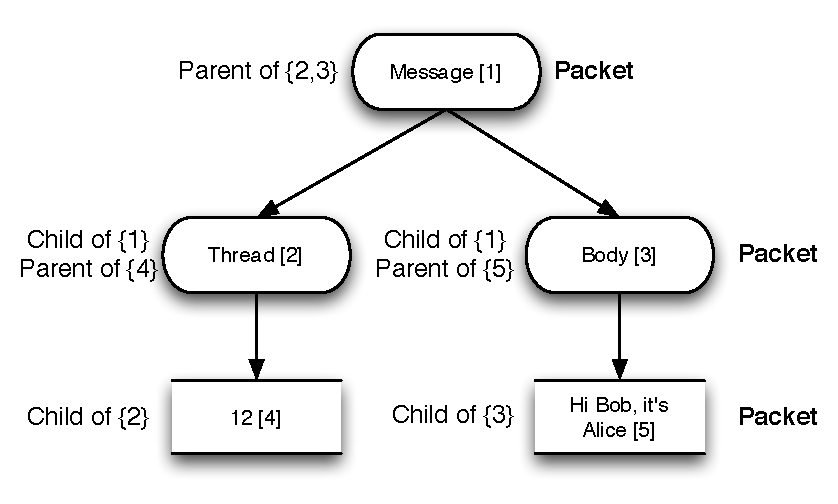
\includegraphics[scale=0.7]{./Figures/Ch6/6-4-4-2.pdf}
    \end{center}
    
    This graphic displays how \verb!Packet! classes represent XML elements and store their children in what is effectively a tree. The corresponding XML would be:
    
    \begin{verbatim}
<message>
  <thread>12</thread>
  <body>Hi Bob, it's Alice</body>
</message>
    \end{verbatim}
    
    The \verb!Packet! class can be simply defined overall as a data structure consisting of a name, and attributes, with a \verb!java.util.LinkedList! of child \verb!Packet!s and a pointer to a parent \verb!Packet!, where applicable.
    
    Packets are parsed and handled on a first come, first served basis. Upon receipt, the \verb!Server! places packets in to a \verb!PacketQueue! where they will be picked out one by one by a running \verb!QueueThread! and handled by an appropriate class. \textsection\ref{subsec:combined} provides an overview of how \verb!Packets!, queues and thread fit together in the overall system.
    
    \verb!Packet! can be found in \emph{com.cyanoryx.uni.enima.net.protocol.xml.Packet}.
    
    \subsubsection{Packet Handling}
    \label{subsubsec:packet_queue}
    
      \paragraph{The PacketQueue} class is a thread-safe (synchronized) class that acts as a wrapper around a \verb!java.util.LinkedList! for storing all incoming packets. It has two methods, \verb!push! and \verb!pull!, the latter removes and returns the packet at the top of the queue, and the former adds a packet to the bottom of the queue. Both, alongside being implemented as synchronized, are thread-safe in that \verb!push! notifies all threads awaiting use of the queue when it is finished add the current packet, and \verb!pull! forces threads to wait if the queue is empty.
      
      \paragraph{The PacketListener} class, or more accurately the interface, provides a notify method implemented by the event handlers (\textsection\ref{subsubsec:handlers}) which allows the \verb!QueueThread! (below) to notify said handlers when a packet is pulled from the queue.
      
      \paragraph{The QueueThread} class is perhaps the most important as it acts as the link between receiving a message and handling it. A \verb!QueueThread! is started when a server is first created, and is passed all the desired event handlers and their XML tag identifiers, which are stored in a \verb!java.util.HashMap!. For example, the \verb!OpenStreamHandler! is required to handle new connection requests, signified by \verb!<stream>! and as such its identifier is ``stream." The \verb!QueueThread! is constantly running alongside the server, looking for new packets pushed on to the queue. When it notices a new packet, it pulls it out of the queue and checks the element name of the packet and looks for it in its handler \verb!HashMap!. If a handler is found, it is notified and passed the \verb!Packet! object.
      
      The idea for this came from \cite{Shigeoka:2002ys}. \\
      
      \begin{lstlisting}
public void run(){
  for (Packet packet=packetQueue.pull();
       packet!=null;
       packet=packetQueue.pull()) {
    try {
      // Element name to look for.
      // Matches name of listener
      String match = packet.getElement();

      synchronized(packetListeners){
        Iterator<PacketListener> iter = packetListeners.keySet()
                                                       .iterator();
        // Loop through the current set of listeners
        while (iter.hasNext()){
          PacketListener listener = iter.next();
          // Get the name of the tag to match
          String listenerString = packetListeners.get(listener);
          // If the packet's element matches the
          // element for this listener...
          if (listenerString.equals(match)){
            listener.notify(packet); // ..send packet to handlers
          } 
        } 
      } 
    } catch (Exception e){
      e.printStackTrace();
    }
  } 
} 
\end{lstlisting}
      
      \verb!QueueThread! allows many packets to be sent to a server at once, with each being handled in order and none being lost.
    
      \paragraph{The ProcessThread} class is created whenever a new connection is made to the \verb!Server!. As \verb!InputHandler! objects parse an entire XML document, they are tied-up with each connection until the document is complete (i.e. a \verb!</stream>! is sent). Because of this, if we were to use one \verb!InputHandler! per server, only one connection would be possible at any one time. As a solution, \verb!ProcessThread! is created for each connection, which instantiates a new \verb!InputHandler! object and begins the XML processing on the incoming stream.
    
    \subsubsection{Handlers}
    \label{subsubsec:handlers}
    
    Handler classes are where most of the work is done once a packet has been parsed. Four are required for the basic operation of the Enigma protocol:
    
    \begin{enumerate}
      \item \textbf{OpenStreamHandler} -- handles an open stream request and initiates some default settings such as whether or not the conversation will be authenticated -- \verb!<stream>!.
      \item \textbf{CloseStreamHandler} -- gracefully handles closed connections and cleans up \verb!Session! objects -- \verb!</stream>!.
      \item \textbf{AuthHandler} -- handles all authentication and encryption setup, including received public keys, session keys and so on -- \verb!<auth></auth>!.
      \item \textbf{MessageHandler} -- handles all incoming messages, determines who they are from and displays them in the appropriate window -- \verb!<message></message>!.
    \end{enumerate}
    
    Handlers implement the \verb!PacketListener! interface, meaning they are notified whenever the matching packet type is parsed out of the queue. See \textsection\ref{subsubsec:packet_queue} for further details about how \verb!QueueThread! determines which handler to use. Handlers, on creation, also receive a reference to the master \verb!SessionIndex! within \verb!Server!.
    
    The handler implementations can be found at \emph{com.cyanoryx.uni.enigma.server}.
    
    \subsection{Fitting the Protocol Components Together}
    \label{subsec:combined}
    
    So, how do these classes fit together in the final system? We've so far given distinct diagrams, and provided abstract descriptions of classes and how they relate, but this is hard to conceive as a whole system.
    
    \begin{center}
      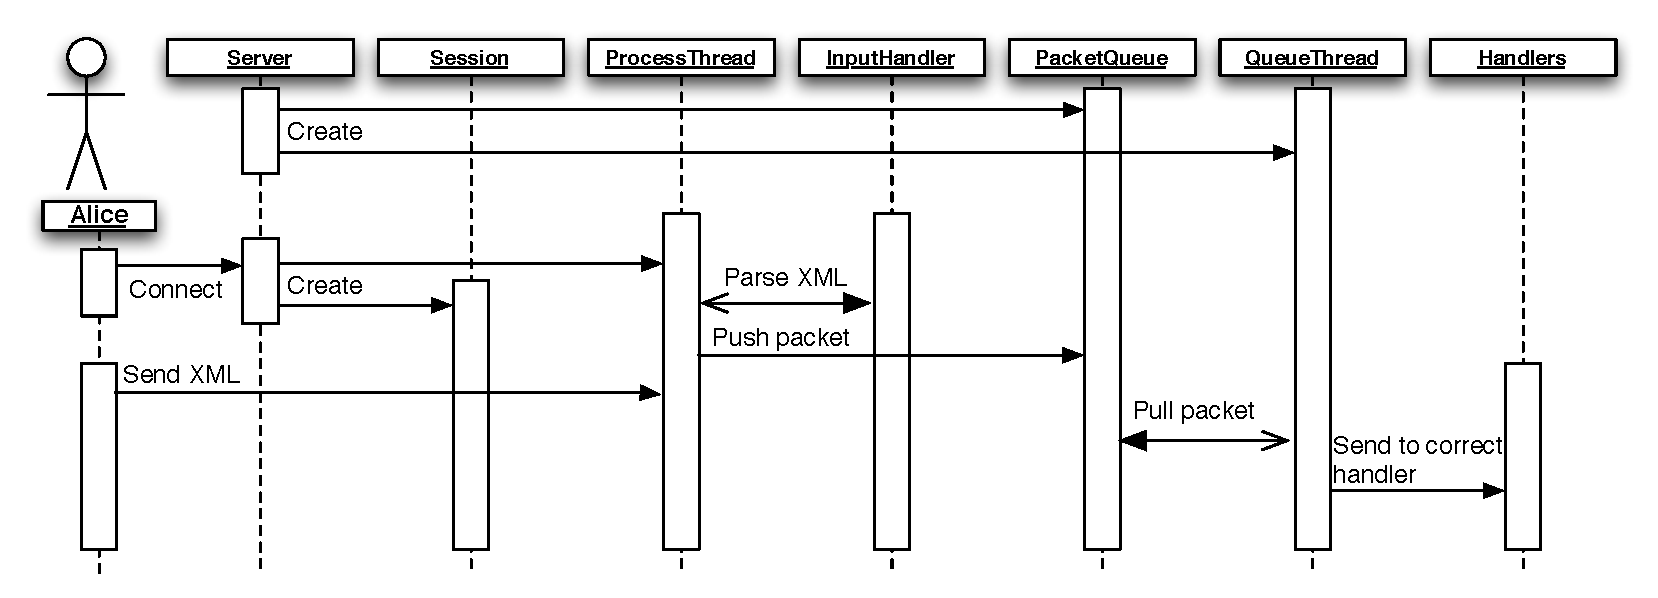
\includegraphics[scale=0.5]{./Figures/Ch6/6-4-5.pdf}
    \end{center}
    
    This figure shows the process of \verb!Server! creation, through to client connection and and message receipt.

\section{Algorithm Implementation}
  \emph{Packages covered in this section: com.cyanoryx.uni.crypto.*}
  
  \subsection{Interfaces and Abstraction}
  
  One of the major points of the Enigma application is the ability to easily introduce new symmetric or asymmetric algorithms in to the application. To do this, we use a well known concept of object-oriented programming: abstraction. Abstraction, in its basic form, is the process of representing some data or logic but hiding the actual implementation. A good example of this is our \verb!LogHandler! earlier, which provides an abstraction of outputting log information -- the developer/program is provided with an interface with, for example, a \verb!log()! method that displays a supplied string in a log window. The implementation of the log function is irrelevant to the developer, all they need to know is that they can use it to reliably log information. Because of this, the logic behind logging data can be changed as necessary assuming it still has the same output -- this is known as a ``black box."
  
  In Java, abstraction is implemented using \emph{interfaces}. An interface defines methods along with their input and output data types, and any class that \emph{implements} this interface must create the logic for these methods. How are interfaces applicable to Enigma? Producing a program that encrypts data using multiple libraries can be difficult as each may have subtle differences in how they expect to receive and output data. For example, a block cipher $A$ may implement a \verb!encrypt()! method that takes portions of data as byte arrays, whereas a cipher $B$ may take the entire plaintext as \verb!String!. To solve this, an interface will be introduced with an \verb!encrypt! method that requires all implementing classes use it -- this results in a standard implementation of all algorithms, meaning a developer knows without a doubt what to input and what to expect back.
  
  This is particularly applicable to Enigma as it means code repetition when dynamically switching between algorithms is reduced significantly. Alongside this, if a new algorithm is desired for use, it simply needs to implement the Enigma encryption interface.
  
  \subsection{Key Agreement and Certficates}
  
  The initiator of a conversation sends their certificate (including their public-key signed by a Certificate Authority) immediately after a successful connection is made. If the certificate is valid and verifiable, the receiver will generate a session key and encrypt it using the initiator's public key before transmitted it. Both users now have a shared session key, and can begin encrypting messages before sending.
  
  This is the standard flow for authentication and key agreement. This takes place primarily in \verb!Connect#connect()! and \verb!AuthHandler#notify()!, which can be found in \emph{com.cyanoryx.uni.enigma.gui} and \emph{com.cyanoryx.uni.enigma.net.server}, respectively.
  
  \paragraph{Key Generation} is performed through an option in the toolbar -- Options $>$ Generate Keys... -- and requires no user input other than having previously set the Certificate Authority's key location in the preferences.
    
  This utility automatically generates a public/private key pair for the user and then signs it with the Certificate Authority's private key to produce their own certificate which will be used by other entities to confirm their identities. In the Real World, users would not have access to the private keys of the CA, however as this application is for research and will not utilise an actual CA we will assume the ownership of CA private keys.
  
  \subsection{Ciphers}
  
  Now that we have a shared session key, messages can now be encrypted by either entity and transmitted over the network securely. 
  
  \paragraph{Sending a message} is handled by \verb!Session#sendMessage()! which will, before sending a message, check to see if the current connection requires encrypted messages and if so it encrypts them using the chosen algorithm. For example, AES: \\
  
  \begin{lstlisting}
AES aes = new AES();
				
Key k = new Key(KeySize.K256);
k.setKey(key);
aes.setKey(k);
			
aes.setPlainText(body.getBytes());
msg=Base64.encodeBytes(aes.encrypt());
\end{lstlisting}

  As can be seen, messages are encoded using Base64 before transmission. Symmetric ciphers encrypt in blocks of bytes, and so trying to send the output from a cipher directly will result in sending binary data which can cause issues within XML documents. Base64 is an encoding scheme that takes binary data and represents it as ASCII text, meaning it can be printed and displayed using almost all character sets. The inner workings of Base64 are out of the scope of this project, however \textsection\ref{AppendixD} lists the open source library used for encoding and decoding.
  
  It should be noted that the actual XML of a message is not encrypted, but only the body.
  
  \paragraph{Receiving a message} is simple, first we must check to see if we are expecting and allowing encrypted messages, and if so create the appropriate cipher object. For example, using AES: \\
  
  \begin{lstlisting}
AES aes = new AES();
Key k = new Key(KeySize.K256);
// Get the session key from the Session object
k.setKey(s.getCipherKey());
aes.setKey(k);
// Convert the Base64 encoded message to binary
aes.setCipherText(Base64.decode(message));
// And decrypt it, producing a String object from the 
// byte array
message = new String(aes.decrypt());
\end{lstlisting}

  The message will then, as usual, be sent to the appropriate conversation window.
  
\section{Testing}

\subsection{Test Driven Development}

A fairly new (or at least recently popular) development methodology was used for the application and algorithms development: test driven development. After creating a basic set of requirements for each unit of code, a test is written for that unit that defines what the input and output should be. Each line of code written should be a response to a part of a test.

Software engineering is often compared to other engineering disciplines, like those that involve bridge building. However these metaphors tend to fall apart as you go deeper. Testing in non-software related engineering fields is difficult -- you have to build the product to test it -- whereas it is easy, even cheap, in software engineering to create tests \emph{before} the product has been built and run them until they pass.

Regularly developers, and even managers, will claim that there is not enough time to test or that it is too much overhead, but if we are to use metaphors anyway we can use them for this: an engineer creating a building cannot simply put off tests because they don't have time, otherwise they endanger lives. Software engineering errors can endanger lives\cite{Leveson:1995aa}, and testing reduces that risk considerably. \emph{Testing is the engineering rigour of software development}\cite{Henney:2010aa}.

\subsection{Unit Testing}	

Being the primary, basic form of testing that most developers use for requirements testing, unit tests are a form of black box testing. This means that all that is taken in to account is the input to and output from the program, thus treating the unit of code as a \emph{black box} where the inner workings cannot be determined. 

Unit tests will be our main method for testing as they are simple and quick to implement, reducing the overhead and supposed time-sink of creating tests.

Each root package in the \verb!com.cyanoryx.uni! tree contains a \emph{test} directory with the appropriate unit tests.

\subsection{Code Coverage}

Code coverage (CC) is a method of measuring how many lines of code in a project are executed during automated testing. It is a useful tool for determining what percentage of an application is covered by tests, meaning that we are able to say whether or not said application is provably working as expected by computing if our passing tests represent the program as a whole.

There are many utilities for calculating this, and in our case an open-source toolkit known as \emph{EMMA}\footnote{http://emma.sourceforge.net/} was used.

\subsection{Functional Testing}

Functional testing is a subset of black box testing that involves (mostly automatically) testing that user interface components work properly and buttons do what they're designed to do. However, it was decided in the case of Enigma that due to the low complexity of the software and use-flow, functional testing could be done manually to ensure that the software worked as properly.

\section{Summary}

We have now listed all the general components that make up the Enigma application: interface, server and algorithms. We will now go on to think about the algorithms and their implementations in further detail -- known as cryptanalysis.

\section{Usage}

  A user's instruction manual is included as \emph{\textsection \ref{AppendixD}}. This manual also briefly covers compilation, required dependencies, and other build related information.

\section{Program Listing}

  Due to the size of the project a detailed, printed code listing is impossible, and thus it is recommended that the code be viewed using a text editor or other text environment on a device. If you do not have a digital copy of this project, please see \emph{\textsection \ref{sec:project_repo}}.